% Template article for document class `jicspack'
% 2004/10/07


\documentclass[print]{jicspack}
\setvolume{11}                             %for printing use only
\setyear{2015}                             %for printing use only
\setpagerange{1}{8}                    %for printing use only
\setheadauthor{X. Liu et al.}          %for printing use only
\setissn{1553--9105} \setpubdate{January 2015} \setno{1}

\afterpage{\beginheader}                   %for printing use only


\usepackage{enumerate}
% if you use PostScript figures in your article
% you can use the graphics package
% \usepackage{graphics}
% or use the graphicx package for more complicated function
\usepackage{graphicx}
% or use the epsfig package
% \usepackage{epsfig}

% The amssymb package provides various useful mathematical symbols
\usepackage{amssymb}

\begin{document}

\begin{premaker}

% The premaker environment contains Title, authors and addresses;
% use the thanksref command within \title, \author or \address for footnotes;
% use the corauthref command within \author for corresponding author footnotes;
% use the ead command for the email address,
% and the form \ead[url] for the home page:
% \title{Title\thanksref{label1}}
% \thanks[label1]{}
% \author{Name\corauthref{cor1}\thanksref{label2}}
% \ead{email address}
% \ead[url]{home page}
% \thanks[label2]{}
% \corauth[cor1]{Corresponding author}
% \address{Address\thanksref{label3}}
% \thanks[label3]{}

\title{An Improved Imputation Method for Missing Data Based on QENNI \thanksref{label1}}
\thanks[label1]{Project supported by the National Nature Science Foundation of China (No. ***).}
\author[author1]{Zhaoyu Zhang\corauthref{cor1}},
\ead{email@address.com}
%\thanks[label2]{Footnotes for authors}
\corauth[cor1]{Corresponding author.}
% other authors
\author[author2]{Zhibo Chen}
\author[author3]{JianXin Wang}

\address[author1]{School of Information Science And Technology, Beijing Forestry University, Beijing 100083, China}
\address[author2]{School of Information Science And Technology, Beijing Forestry University, Beijing 100083, China}
\address[author3]{School of Information Science And Technology, Beijing Forestry University, Beijing 100083, China}
%\thanks[label3]{Footnotes for address}
% you can use optional labels to link authors explicitly to addresses:
% \author[label1]{},
% \author[label2]{}
% \address[label1]{}
% \address[label2]{}

\begin{abstract}
% Text of abstract
This article is designed to help in the contribution for the Journal of Computational Information Science.
It is divided into several sections.
Section 1 consists of the styles and notes for the main text.
Section 2 illustrates the Mathematical writing style.
Section 3 and 4 cover the topic of drawing tables and inserting figures respectively.
The residuals deal with references, appendix, acknowledges, etc.
\end{abstract}
\begin{keyword}
% keywords here, in the form: keyword \sep keyword
Style guide \sep Examples \sep Latex style
\end{keyword}
\end{premaker}

% main text
\section{Main Text}
\label{Maintext}
\begin{itemize}
\item{\bf Common} Contributions must be written in English. Each
paper should be introduced by a list of keywords and a
self-contained abstract of no more than thirty lines without long
formulas. \item{\bf Title} Title should be concise but
informative. Titles are often used in information-retrieval
systems. Avoid abbreviations and formulae where possible.
\item{\bf Author} There should be and should only be one
corresponding author. \item{\bf Abstract} A concise and factual
abstract, of around 100 words, is required. The abstract should
state briefly the purpose of the research, the principal results
and major conclusions. It must be able to stand alone, references
should be avoided. Non-standard or uncommon abbreviations should
be avoided. \item{\bf Keywords} Three to five keywords are
required, using British spelling and avoiding general and plural
terms and multiple concepts (avoid, for example, ``and", ``of").
\item{\bf Headings} Papers should be divided into numbered
sections, subsections and, if necessary, subsubsections (e.g. 3,
3.1, 3.1.1, etc.). \item{\bf Uppercase \& Lowercase} Every word
within the title of ``section" , except empty word, should has its
initial capitalized. But for the ``subsection" , the only word
that should be capitalized is the first one. But note that it is
not the case for subsection, see subsection
\ref{subsectiontitlerule}. \item{\bf Mathematical Symbols} Every
mathematical symbol in the text, for example, $n, R, x, y$ etc.
\item{\bf Enumerations} Enumerations should be listed in an
Item-like environment, e.g. ``itemize" ``enumerate". \item{\bf
Footnotes} Footnotes should be avoided if possible and as brief as
possible, they should be numbered consecutively. \item{\bf
Algorithms} If you are presenting an algorithm or listing
something with order, make sure you use the ``itemize" or
``enumerate"  environment, treat each step as an ``item" and label
it as ``($n$)", where $n$ is the sequence number of steps. For the
sub-items label them as ``a.", ``b." , etc., see section
\ref{sec:1.1}. \item{\bf Figures} Figures should be numbered
consecutively in the order of appearance and citation in the text.
Be sure to cite every figure. Handwritten lettering and
low-quality computer graphics are not acceptable. EPS electronic
files should be sized as they will appear in the journal.
\item{\bf Tables} Tables must be numbered and typed on separate
pages. The table title, which should be brief, goes above the
table. Detailed explanations or table footnotes should be typed
directly beneath the table. Note that tables are usually typeset,
not scanned (tables cannot be electronically reduced in size).
\item{\bf Citations} Citations should coupled with labels. That
is, to make a citation , you should label the position first, then
use the command ``\verb|\ref|". All citations made in this guide,
including equations, tables, figures, etc., follow this rule, you
can check the source file to make a clearer understood. \item{\bf
References} References must be numbered consecutively in the order
of their first citation, as in the following examples: books
\cite{NumeApp,texbook}, articles in journals \cite{UncaliEu},
papers in a contributed volume \cite{Deformation,canonical},
unpublished papers \cite{SpaceDeform}.
\end{itemize}
\subsection{Only the first word in the title of ``subsection" be capitalized}
\label{sec:1.1}
We place a paradigm for the algorithm here:
\begin{enumerate}[(1)]
\item The first step.
\item The second step.
  \begin{enumerate}[a.]
  \item substep1.
  \item substep2.
  \end{enumerate}
\item  The last step.
\end{enumerate}
In the ``.tex" file it may look like the following:
\begin{verbatim}
\begin{enumerate}[(1)]
\item The first step.
\item The second step.
  \begin{enumerate}[a.]
  \item substep1.
  \item substep2.
  \end{enumerate}
\item  The last step.
\end{enumerate}
\end{verbatim}

You can also use description environment, for example
\begin{description}
\item[Step 1] The first step. \item[Step 2] The second step.
\item[Step 3] The second Step.
\end{description}
In the ``.tex" file it may look like the following:
\begin{verbatim}
\item[Step 1] The first step.
\item[Step 2] The second step.
\item[Step 3] The second Step.
\end{verbatim}
{\bf Note:} Package ``enumerate" is needed for this kind of usage
of environment of enumerate. \label{subsectiontitlerule}
\section{Mathematical Notation}
\subsection{Build-in environments}
This document class has provided you some commonly used environments:
\begin{itemize}
\item{Definition environment}\\
{\verb|\begin{defn}|
$\cdots\cdots$
\verb|\end{defn}|}
\item{Lemma environment}\\
{\verb|\begin{lem}|
$\cdots\cdots$
\verb|\end{lem}|}
\item{Theorem environment}\\
{\verb|\begin{thm}|
$\cdots\cdots$
\verb|\end{thm}|}
\item{Proof environment}\\
{\verb|\begin{pf*}{Proof}|
$\cdots\cdots$ \verb|\end{pf*}|}
\item{Corollary environment}\\
{\verb|\begin{col}|
$\cdots\cdots$
\verb|\end{col}|}
\item{Proposition environment}\\
{\verb|\begin{pro}|
$\cdots\cdots$
\verb|\end{pro}|}
\end{itemize}

The following examples demonstrate the usage of the above environments.
\begin{defn}
A graph $G$ is an ordered pair of disjoint sets $(V,E)$ such that $E$ is a subset of the set
of unordered pairs of $V$.
\end{defn}
\begin{lem}
If $m\geqslant 2n$ then $\epsilon(\overrightarrow{G};x,y)=0$.
\end{lem}


\begin{thm}
A graph is bipartite if it does not contain an odd cycle.
\end{thm}
\begin{pf*}{Proof}
Suppose $G$ is bipartite with vertex classes $V_1$ and $V_2$.
Let $x_1x_2\cdots x_l$ be a cycle in $G$.
We may assume that $x_1\in V_1$. Then $x_2\in V_2$, $x_3\in V_1$,and so on:
$x_i\in V_1$ if $i$ is odd.
Since $x_l\in V_2$, we find that $l$ is even.\\
\indent{}Suppose now that $G$ does not contain an odd cycle. Since a graph is bipartite if each component of it is,
we may assume that $G$ is connected. Pick a vertex $x\in V(G)$ and put $V_1=\{y| d(x,y)\mbox{is odd}\}$,
$V_2=V\backslash V$. There is no edge joining two vertices of the same class $V_i$ since otherwise $G$ would contain an odd cycle.
Hence $G$ is bipartite.
\end{pf*}
\begin{thm}
A graph is a forest if for every pair $\{x,y\}$ of distinct vertices it contains at most one $x$-$y$ path.
\end{thm}
\begin{pf*}{Proof}
If $x_1x_2\cdots x_l$ is a cycle in a graph $G$ then $x_1x_2\cdots x_l$ and $x_1x_l$ are two $x_1$-$x_l$ paths in $G$.\\
\indent{}Conversely, let $P_1=x_0x_1\cdots x_l$ and
$P_2=x_0y_1y_2\cdots y_kx_l$be two distinct $x_0$-$x_l$ paths in a
graph $G$. Let $i+1$ be the minimal index for which $x_{i+1}\neq
y_{i+1}$, and let $j$ be the minimal index for which $j\geqslant
i$ and $y_{j+1}$ is a vertex of $P_1$, say $y_{j+1}=x_h$. Then
$x_ix_{i+1}\cdots x_ky_jy_{j-1}\cdots y_{i+1}$ is a cycle in $G$.
\end{pf*}
\begin{col}
Every connected graph contains a spanning tree, that is a tree containing every vertex of the graph.
\end{col}
\begin{pf*}{Proof}
Take a minimal connected spanning subgraph.
\end{pf*}
\begin{col}
A tree of order $n$ has size $n-1$; a forest of order $n$ with $k$ components has size $n-k$.
\end{col}
\begin{defn}
An oriented graph is a directed graph obtained by orienting the edges,
that is by giving the edge $ab$ a direction $\overrightarrow{ab}$ or $\overrightarrow{ba}$.
Thus an oriented graph is a directed graph in which at most one of $\overrightarrow{ab}$ and $\overrightarrow{ba}$ occurs.
\end{defn}
\begin{pro}
The set
$$S_m^\mu(\Delta)=\{f|\  {\rm deg} f\leqslant m, f\in S_m^\mu(\Delta)\}$$
is a finite-dimensional linear vector space on $k$, $m\geqslant
0$.
\end{pro}
\begin{lem}
$G$ is Hamiltonian if $C_n(G)$is and $G$ has a Hamilton path if so does $C_{n-1}(G)$.
\end{lem}
{\bf Note:} If you use the above environments, it will be numbered
automatically. If the above environments failed to prove their
sufficiency, feel free to define your own theorem-like
environments, i.e. \verb|\newtheorem\{Name\}\{Caption\}|.
%Make sure that all of your arrays display in the displaystyle.
\subsection{Equations}
\label{equsection}
%We recommend that you follow the following rules to make your article more readable and intelligible.
%Lengthy equations should be placed in the Mathematical environment, i.e. \verb|$$ $$| or \verb|\begin\{math\}| $\cdots$ \verb|\end\{math\}|.
Here are some examples of equations that cover the rules of making a equation with explanations following.

Expressions that are too long or oversized should be separated
from the main text, i.e. be surrounded by
\verb|$$|$\cdots$\verb|$$|. For example,
$$
f(x)=\sum\limits_{k=1}\limits^{\infty}c_kT_{3^k}(x).$$

Never try to number the equation manually. If you want to number a
equation, use the corresponding environment, i.e. \verb|Equation|
or \verb|Eqnarray| if you want to display mutiple equations with
numbers. Eq. (\ref{eq:1}, \ref{eq:2})  and Eq. (\ref{eq:3})
demonstrate the usage of \verb|Equation| and \verb|Eqnarray|
environments respectively.
\begin{equation}\label{eq:1}
p(x)=a_0+a_1+\cdots+a_nx^n.
\end{equation}
\begin{equation}\label{eq:2}
[L/M]=\frac
{\left|
\begin{array}{cccc}
a_{L-M+1} & a_{L-M+2} & \cdots & a_{L+1}\\
\vdots & \vdots &  & \vdots\\
a_{L} & a_{L+1} & \cdots & a_{L+M}\\
\sum\limits_{j=M}\limits^{L}a_{j-M}{X^j} & \sum\limits_{j=M-1}\limits^{L}a_{j-M+1}{X^j} & \cdots & \sum\limits_{j=0}\limits^{L}a_{j}{X^j}\end{array}
\right|}
{\left|
\begin{array}{cccc}
a_{L-M+1} & a_{L-M+2} & \cdots & a_{L+1}\\
\vdots & \vdots &  & \vdots\\
a_{L} & a_{L+1} & \cdots & a_{L+M}\\
x^{M} & x^{M-1} & \cdots & 1
\end{array}
\right|}.
\end{equation}
\begin{eqnarray}\label{eq:3}
K_m(t)&=&\frac{1}{(m-1)!}E((x-t)_{+}^{m-1};\alpha)\nonumber\\
      &=&\frac{1}{(m-1)!}\left((\alpha-t)_{+}^{m-1}-\sum\limits_{k=0}\limits^{n}l_k(\alpha)(x_k-t)_{+}^{m-1}\right).
\end{eqnarray}

Use \verb|displaystyle|  to make formulas bigger when necessary.
\begin{equation}\label{eq:4}
f(z)\thickapprox\frac{\displaystyle 1+\frac{1}{2}z+z^2+\frac{1}{2}z^3}{\displaystyle 1-\frac{1}{2}z+z^2}.
\end{equation}

The texts in the equations should not be writing in the
mathematical form, you can use \verb|\mbox{#text}| to achieve
this, example is given in Eq. (\ref{eq:5}).


\begin{eqnarray}\label{eq:5}
f(x)=\left\{\begin{array}{ll}3x^2 & \mbox{when}\ x\geqslant 0,\\-3x^2 & \mbox{when}\ x\leqslant 0.\end{array}\right.
\end{eqnarray}

When dealing with well-known functions like min, sin, cos , etc.,
you should use their normal form in the math environment, i.e. use
\verb|\min, \sin, \cos,| $\cdots$ respectively.
$$\arg\min\{\sin{x}\times\cos(x)\}$$
$$\arg\min\{\sin{x}\times\cos(x)+f(x)-g(x)+e(x)\},$$

If a sentence is not ended at a equation, the words follows the
sentence may not be initial capitalized and intend, see Eq.
(\ref{eq:6}).

 Then the unconditional pdf of $X$ is
\begin{equation}\label{eq:6}
f_X(x)=\int f_{X|\Theta}(x|\theta)f_{\Theta}(\theta)d\theta,
\end{equation}
where the integral is taken over all values of $\theta$ with positive probability.
\section{Table Section}
Use ``Table" or ``Tabular" environment as usual. You may center
the table most of the time to beautify your article. You also
should name each table. Table [\ref{lab:1}, \ref{lab:2}] are two
typical examples of tables.
\begin{table}[h]
\centering \caption{Observation results for LSE} \label{lab:1}
\begin{tabular}{|c|c|c|c|c|c|c|c|c|}
\hline $k$   & 1 & 2 & 3 & 4 & 5 & 6 & 7 & 8\\
\hline $x_k$ & 0 & 1 & 2 & 3 & 4 & 5 & 6 & 7\\
\hline $y_k$ & 1.4 & 1.3 & 1.4 & 1.1 & 1.3 & 1.8 & 1.6 & 2.3\\
\hline
\end{tabular}
\end{table}
\begin{table}[h]
\centering \caption{Primitive types in Java}
\label{lab:2}
\begin{tabular}{|c|c|c|c|c|}
\hline
Primitive type & Size & Minimum & Maximum & Wrapper type\\\hline
boolean & -- & -- & -- & Boolean\\\hline
char & 16-bit & Unicode 0 & Unicode $2^{16}-1$ & Character\\\hline
byte & 8-bit & -128 & +127 & Byte\\\hline
short & 16-bit & $-2^{15}$ & $+2^{15}-1$ & Short\\\hline
int & 32-bit & $-2^{31}$ & $+2^{31}-1$ & Integar\\\hline
long & 64-bit & $-2^{63}$ & $+2^{63}-1$ & Long\\\hline
float & 32-bit & IEEE754 & IEEE754 & Float\\\hline
double & 64-bit & IEEE754 & IEEE754 & Double\\\hline
void & -- & -- & -- & Void\\\hline
\end{tabular}
\end{table}
\section{Figure Section}
\label{Figuresection}
If you have figures, include them like this:
\begin{figure}[h]
\centering
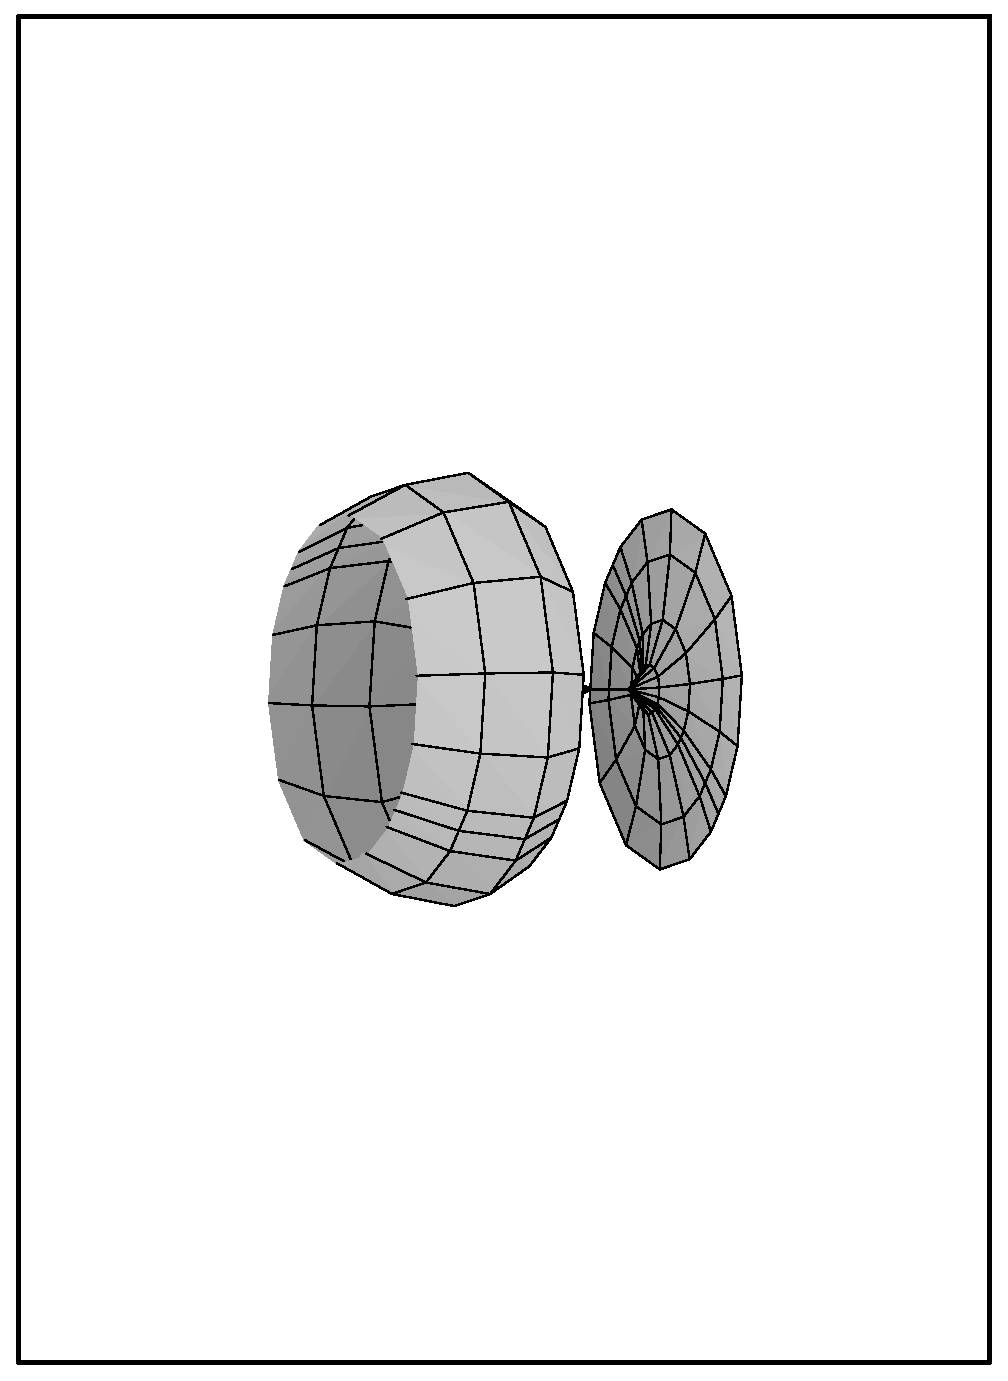
\includegraphics[angle=-90, width=0.3\textwidth]{cup1.eps}
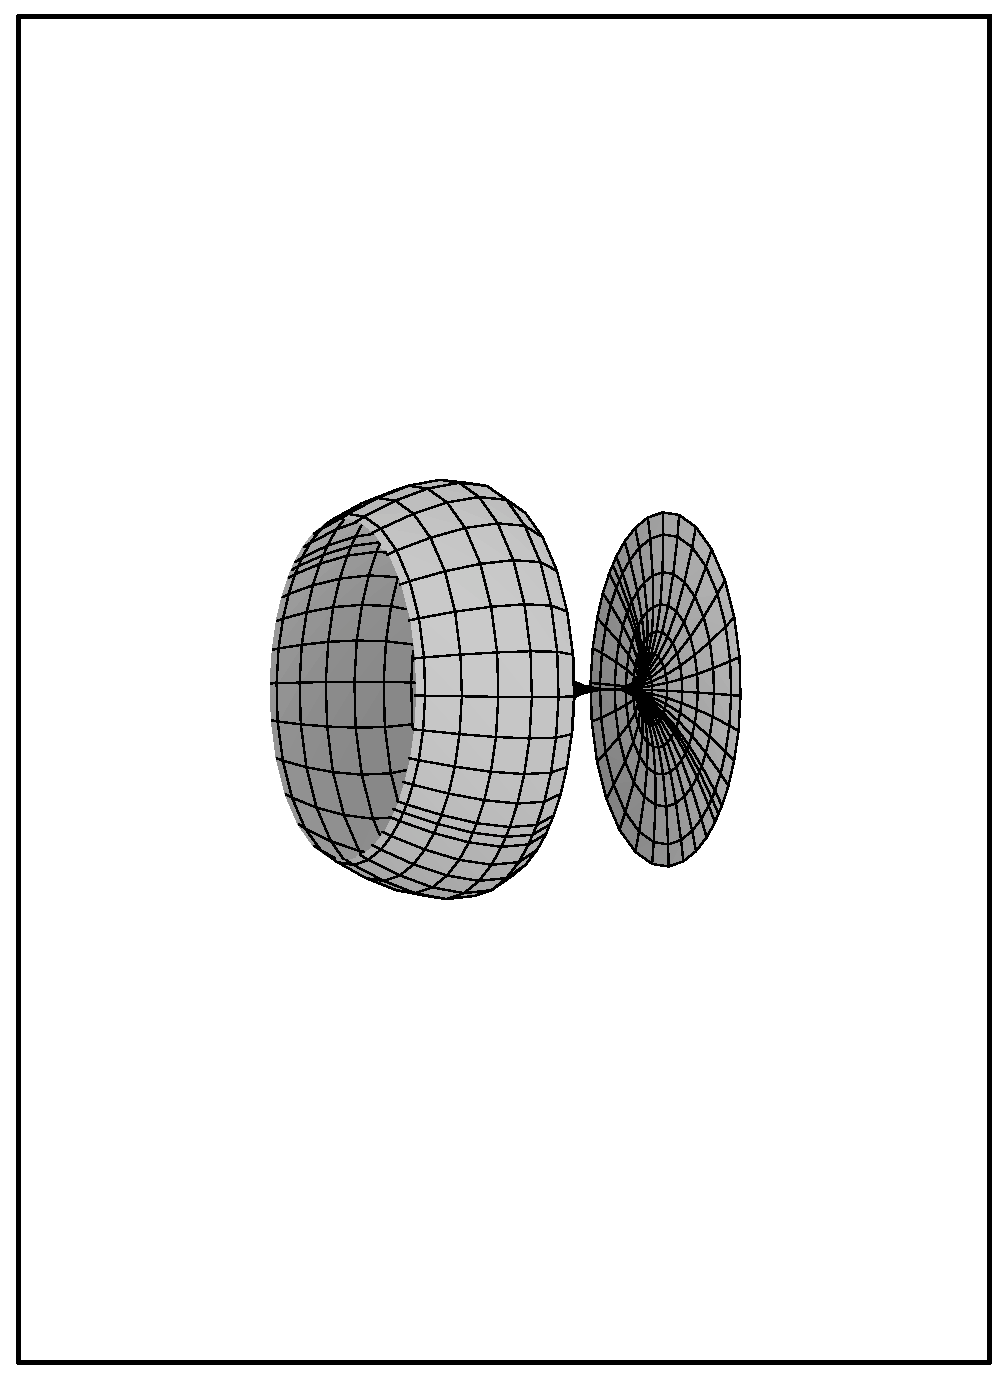
\includegraphics[angle=-90, width=0.3\textwidth]{cup2.eps}
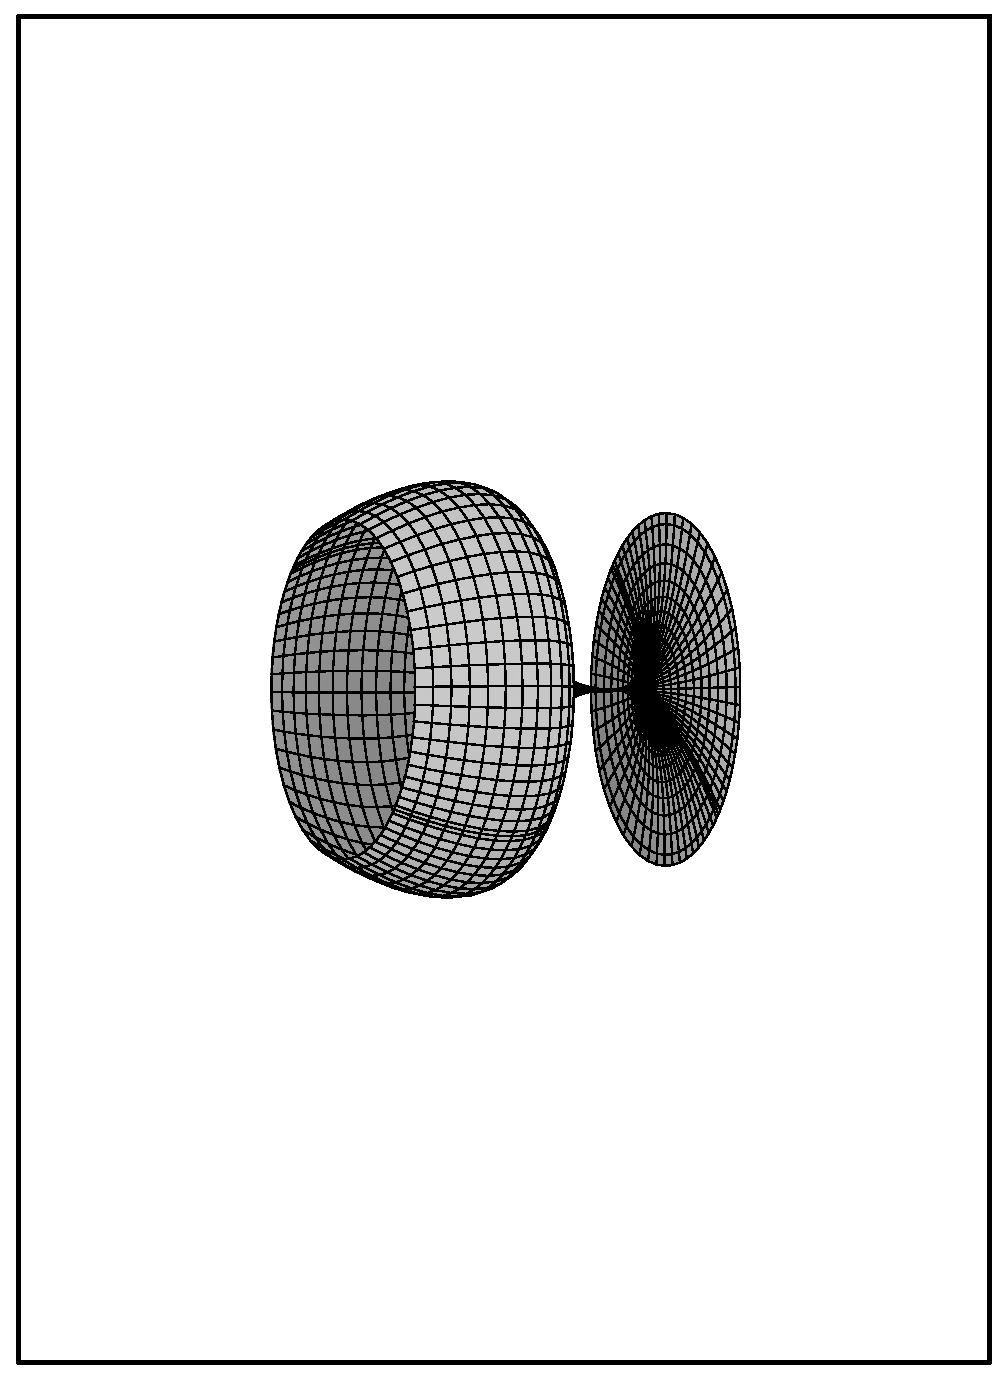
\includegraphics[angle=-90, width=0.3\textwidth]{cup3.eps}

\caption{The control polygon sequences of a cup-like rotation}
\label{fig:levfig}
\end{figure}

You can then cite them in your article as following: Fig.
\ref{fig:levfig} shows a process of level set based segmentation.



\section{Citing a Reference}
You can cite a reference by making use of the command ``\verb|\cite|" after you have labelled a bibliography\cite{labelbib}.
An illustration of \TeX/\LaTeX in given in \cite{texbook}.
Please refer to \cite{NumeApp,UncaliEu,SpaceDeform,Deformation} to get a detailed format of references.
The citation in the former sentence can be made by using the command ``\verb|\cite{|\verb|NumeApp|, \verb|UncaliEu|, \verb|SpaceDeform|, \verb|Deformation}|", where NumApp, UncaliEu, etc., are user defined labels for references.
% appendix sections are done as normal sections

\section*{Acknowledgement}
Acknowledge here.
\section*{Appendix} Appendix here.
\begin{thebibliography}{00}\label{ref:ref}

% \bibitem{label}
% Text of bibliographic item

% notes:
% \bibitem{label} \note

% subbibitems:
% \begin{subbibitems}{label}
% \bibitem{label1}
% \bibitem{label2}
% If there is a note, it should come last:
% \bibitem{label3} \note
% \end{subbibitems}

\bibitem{labelbib} Bibliography, For further detail, please visit our
website, http://www.joics.com, 2004
\bibitem{NumeApp} R. H. Wang, {\it Numerical Approximation}, Higher Education Press, Beijing, 1999
\bibitem{UncaliEu} A. Fusiello, Uncalibrated euclidean reconstruction: a review, Image and Vision Computing 18 (2000) 555-563
\bibitem{Deformation} X. Provot, Deformation constraints in a mass-spring model to describe rigid cloth behavior, in: Proc. Graphics Interface '95, 1995, pp. 147-154
\bibitem{SpaceDeform} Y. Sun, Space Deformation with Geometric Constraint, M. S. Thesis, Department of Applied Mathematics, Dalian University of Technology, March 2002
\bibitem{texbook} Donald E. Knuth, {\it The TEXbook}, Addison--Welsey, 1996
\bibitem{canonical}E. L. Ortiz, Canonical polynomials in the Lanczos tau-method, in: B. Scaife (Ed.), Studies in Numerical Analysis, Academic Press, New York, 1974, pp. 73-93
\end{thebibliography}

\end{document}
